\label{ch:advection}


\section{The linear advection equation}

The linear advection equation is simply:
\begin{equation}
\label{eq:advect}
a_t + u a_x = 0
\end{equation}
where $a(x,t)$ is some scalar quantity and $u$ is the velocity at
which it is advected ($u > 0$ advects to the right).  The solution to
Eq.~\ref{eq:advect} is to simply take the initial data, $a(x,t=0)$,
and displace it to the right at a speed $u$.  The shape of the initial
data is preserved in the advection.  Many hyperbolic systems of PDEs,
e.g.\ the equations of hydrodynamics, can be written in a form that
looks like a system of (nonlinear) advection equations, so the
advection equation provides important insight into the methods used
for these systems.
%
\begin{exercise}[Linear advection analytic solution]
{Show via substitution that $a(x - ut)$ is a solution to
  Eq.~\ref{eq:advect} for any choice of a.  This means that
the solution is constant along the lines $x = u t$
(the curves along which the solution is constant are called the
characteristics).}
\end{exercise}

Figure~\ref{fig:advection_char} shows an initial profile, $a(x)$, and
the corresponding characteristics in the $t$-$x$ plane.  With time,
since the solution is constant along these characteristics, it simply
each point simply follows the characteristic curve, resulting in a
shift of the profile to the right.

An important concept that we will discuss shortly is {\em stability}.
Not every discretization that we write down will be well behaved.  For
some, our initial state will begin to ``blow-up'', and take on
obscenely large and unphysical values after just a few steps.  This is
the hallmark of a method that is unstable.  Some methods have
restrictions on the size of the timestep that result in a stable
methods as well.

% this figure is produced by figures/advection/characteristics.py
\begin{figure}[t]
\centering
\includegraphics[width=0.6\linewidth]{advection-characteristics}
\caption[Characteristics for linear advection]
{\label{fig:advection_char} (top) Initially sinusoidal
distribution (bottom) Characteristic
structure for the linear advection equation $u = 1$.  Note
that for this linear equation the characteristics are all parallel
(they have the same slope in the $t$-$x$ plane.}
\end{figure}

\section{First-order advection in 1-d and finite-differences}

To get a flavor of the methods for advection, we will use a simple
finite-difference discretization---here, the domain is divided into
a sequence of points where we store the solution.
We will solve
Eq.~\ref{eq:advect} numerically by discretizing the solution at
these points.  The index $i$ denotes the point's location, and $a_i$
denotes the discrete value of $a(x)$ in zone $i$.  The data in each
zone can be initialized as $a_i = a(x_i)$.  Figure~\ref{fig:fdgrid}
shows the grid.

We also need to discretize in time.  We denote the time-level of the
solution with a superscript, so $a_i^n = a(x_i,t^n)$.  For a fixed
$\Delta t$, time level $n$ corresponds to a time of $t = n\Delta t$.


A simple first-order accurate discretization is:
\begin{equation}
\frac{a_i^{n+1} - a_i^n}{\Delta t} = - u \frac{a_i^n - a_{i-1}^n}{\Delta x}
\label{eq:fo}
\end{equation}
This is an {\em explicit} method, since the new solution, $a_i^{n+1}$,
depends only on information at the old time level, $n$.  

Finally, we also need to specify a boundary condition for this.  Our
choice of spatial derivative is one-sided---it uses information from
the zone to the left of the zone we are updating.  This is because
information is flowing from left to right in this problem ($u > 0$).
This choice of the derivative is called {\em upwinding}---this choice
of derivative results in a stable method.
Notice that if we use Eq.~\ref{eq:fo} to update the data in the first
zone inside the boundary, we need data to the left of this
zone---outside of the domain.  This means that we need a single
{\em ghost point} to implement the boundary conditions for our method.  The
presence of the ghost points allow us to use the same update equation
(e.g.\ Eq.~\ref{eq:fo}) for all zones in the domain.


% figure created by figures/advection/fd-ghost.py
\begin{figure}[t]
\centering
\includegraphics[width=\linewidth]{fd_ghost}
\caption[A simple finite-difference grid]{\label{fig:fdgrid} A simple
  finite-difference grid.  The solution is stored at each of the
  labeled points.  The dotted lines show the ghost points used to
  extend our grid past the physical boundaries to accommodate boundary
  conditions.  Note that if we are periodic, then points $0$ and $N-1$
  are at the same physical point in space, so we would only need to
  update one of them.}
\end{figure}

The last piece of information needed to update the solution is the
timestep, $\Delta t$.  It can be shown that for the solution to be
{\em stable}, the timestep must be less than the time it takes information
to propagate across a single zone.  That is:
\begin{equation}
\Delta t \le \frac{\Delta x}{u} \enskip .
\end{equation}
This is called the {\em Courant-Friedrichs-Lewy} or {\em CFL}
condition.  A dimensionless quantity called the {\em CFL number} is 
defined as 
\begin{equation}
\cfl = \frac{\Delta t u }{\Delta x} 
\end{equation}
Stability requires $\cfl \le 1$.
%
We traditionally write the timestep as
\begin{equation}
\label{eq:timestep}
\Delta t = \cfl \frac{\Delta x}{u}
\end{equation}
and specify $\cfl$ as part of the problem (a typical value may be $\cfl = 0.7$).

\begin{exercise}[Perfect advection with a Courant number of 1]
{Show analytically that when you use $\cfl=1$ in the
  first-order differenced advection equation (Eq.~\ref{eq:fo}) that
  you advect the profile exactly, without any numerical error.}
\end{exercise}

Keep in mind that, in general, we will be solving a non-linear
system of equations, so it is not possible to run with $\cfl=1$, 
since $u$ (and therefore $\cfl$) will change from zone to zone.
Instead, one looks at the most restrictive timestep over all the
zones and uses that for the entire system.


\begin{exercise}[A 1-d finite-difference solver for linear advection]
{Write a code to solve the 1-d linear advection equation
  using the discretization of Eq.~\ref{eq:fo} on the domain $[0,1]$ with
  $u=1$ and periodic boundary conditions.  For initial conditions,
  try both a Gaussian profile and a top-hat:}
  \begin{equation}
  a = \left \{
      \begin{array}{lllll}0 & \mathit{~if~~} &         &x& < 1/3 \\
                          1 & \mathit{~if~~} & 1/3 \le &x& < 2/3 \\
                          0 & \mathit{~if~~} & 2/3 \le &x&
      \end{array}
      \right .
  \end{equation}

  \noindent Note: For a general treatment of boundary conditions, you would
    initialize the ghost points to their corresponding periodic data
    and apply the difference equations to zones $0, \ldots, N-1$.
    However, for periodic BCs on this grid, points $0$ and $N-1$ are
    identical, so you could do the update in this special case on
    points $1, \ldots, N-1$ without the need for ghost points and then
    set $a_0 = a_{N-1}$ after the update. \\

  \noindent Run you program for one or more periods (one period
    is $T=1/u$) with several different CFL numbers and notice that
    there is substantial numerical dissipation (see Figure~\ref{fig:fdadvect}).
\end{exercise}

\begin{figure}[t]
\centering
% figure generated by hydro_examples/advection/fdadvect.py
\includegraphics[width=0.8\linewidth]{fdadvect-upwind}
\caption[First-order finite-difference solution to linear advection]
{\label{fig:fdadvect} Finite-difference solution to the first-order
finite-difference upwind method for advection, using 65 points and
a variety of CFL numbers. \\
\hydroexdoit{\href{https://github.com/zingale/hydro_examples/blob/master/advection/fdadvect.py}{fdadvect.py}}}
\end{figure}
%
This method is first-order accurate.  


Ultimately we will want higher-order accurate methods.  The most obvious
change from our initial discretization is to try a higher-order spatial
derivative.

\begin{exercise}[FTCS and stability]
{You may think that using a centered-difference for
  the spatial derivative, $a_x \sim (a_{i+1} - a_{i-1})/(2 \Delta x)$
  would be more accurate.  This method is called FTCS (forward-time,
  centered-space).  Try this on the same test problems.}
\end{exercise}

\begin{figure}[t]
\centering
% figure generated by hydro_examples/advection/fdadvect.py
\includegraphics[width=0.48\linewidth]{fdadvect-FTCS-C0_1}
\includegraphics[width=0.48\linewidth]{fdadvect-FTCS-C0_5}
\caption[FTCS finite-difference solution to linear advection]
{\label{fig:fdadvect-ftcs} Finite-difference solution using the FTCS
finite-difference method for advection using 65 points, modeling for
only 1/10$^\mathrm{th}$ of a period.  The panel of the left is
with $\cfl = 0.1$ and the panel on the right is $\cfl = 0.5$.\\
\hydroexdoit{\href{https://github.com/zingale/hydro_examples/blob/master/advection/fdadvect.py}{fdadvect.py}}}
\end{figure}

You will find that no matter what value of $\cfl$ you choose with the
FTCS method, the solution is unconditionally {\em unstable} (see
Figure~\ref{fig:fdadvect-ftcs}).  If you continue to evolve the
equation with this method, you would find that the amplitude grows
without bound.  There is something about that discretization that
simply gets the physics wrong.


\section{Stability}

\MarginPar{add a discussion of domain of dependence}

The classic method for understanding stability is to consider the growth 
of a single Fourier mode in our discretization.  That is, substitute in
$a_i^n = A^n e^{Ii\theta}$, where $I = \sqrt{-1}$\footnote{our use of $i$ and $j$ as spatial indices presents an unfortunate clash of notation here, hence the use of $I$ for the imaginary unit}, and $\theta$ represents a
phase.  A method is stable if $|A^{n+1}/A^n| \le 1$.  FTCS appears as:
\begin{equation}
  a_i^{n +1} = a_i^n - \frac{\cfl}{2} (a_{i+1}^n - a_{i-1}^n)
\end{equation}
Examining a Fourier mode shows that:
\begin{align}
  A^{n+1}e^{Ii\theta} &= A^n e^{Ii\theta} - \frac{\cfl}{2} \left (
      A^n e^{I(i+1)\theta} - A^n e^{I(i-1)\theta} \right ) \\
  A^{n+1} &= A^n  - \frac{\cfl}{2} A^n \left ( e^{I\theta} - e^{-I\theta}\right ) \\
  A^{n+1} &= A^n \left ( 1 - I \cfl \sin\theta \right )
\end{align}
so the magnitude of the amplification is
\begin{equation}
 \left | \frac{A^{n+1}}{A^n}\right |^2 = 1 + \cfl^2\sin^2\theta
\end{equation}
We see that there is no value of $\cfl$ that can make the method stable
($|A^{n+1}/A^n| > 1$ always).  Doing the same analysis for
Eq.~\ref{eq:fo} would show that the upwind method is stable for $0\le
\cfl \le 1$. 

\begin{exercise}[Stability of the upwind method]
{Using the above stability analysis, considering the amplitude of a
  single Fourier mode, show that the growth of a mode for the upwind
  method (Eq.~\ref{eq:fo}) is:
  \begin{equation}
    \left | \frac{A^{n+1}}{A^n} \right |^2 = 
           1 - 2\cfl(1-\cfl)(1-\cos\theta)
  \end{equation}
  and stability requires $2\cfl(1-\cfl) \ge 0$ or $0 \le \cfl \le 1$.
}
\end{exercise}

It is important to note that this stability analysis only works for
linear equations, where the different Fourier modes are decoupled,
nevertheless, we use its ideas for nonlinear advection problems as
well.

Truncation analysis can also help us understand stability.  The idea
here is to keep the higher order terms in the Taylor series to understand
how they modify the actual equation you are trying to solve.

\begin{exercise}[Stability analysis]
{To get an alternate feel for stability, we can ask
  what the terms left out by truncation look like.  That is, we can
  begin with the discretized equation:
\begin{equation}
  a_i^{n+1} - a_i^n = -\frac{u \Delta t}{\Delta x} ( a_i^n - a_{i-1}^n )
\end{equation}
and replace $a_i^{n+1}$ with a Taylor expansion in time, and replace
$a_{i-1}^n$ with a Taylor expansion in space, keeping terms to
$O(\Delta t^3)$ and $O(\Delta x^3)$.  Replacing $\partial a/\partial t$
with $-u \partial a/ \partial x$ in the higher-order terms, show 
that our difference equation more closely corresponds to 
\begin{eqnarray}
\label{eq:advect_trunc_analysis}
a_t + u a_x &=& \frac{u \Delta x}{2} \left ( 1 - \frac{\Delta t u}{\Delta x} \right ) \frac{\partial^2 a}{\partial x^2} \\
            &=& \frac{u \Delta x}{2} (1 - \cfl) \frac{\partial^2 a}{\partial x^2}
\end{eqnarray}
}
\end{exercise}


Notice that the righthand side of Eq.~\ref{eq:advect_trunc_analysis}
looks like a diffusion term, however, if $\cfl > 1$, then the coefficient
of the diffusion is negative---this is unphysical.  This means that
the diffusion would act to take smooth features and make them more
strongly peaked---the opposite of physical diffusion.

For FTCS, a similar truncation analysis would show that the diffusion term
is always negative.

\subsection{Domain of dependence}

Another important view of our numerical difference scheme is to look
at the {\em domain of dependence}.  Figure~\ref{fig:adv:domains}
illustrates this for the updated point $a_i^{n+1}$ (shown at the top
of center of the space-time diagram).  The numerical domain of
dependence shows the points that can influence the updated value of
$a_i$ using our difference method.  For the upwind scheme, we see that
this is a triangle that includes $a_{i-1}^n$ and $a_i^n$.  The
physical domain of dependence is shown as the orange triangle---this
is formed by tracing backwards in time from $a_i^{n+1}$ along a
characteristic, reaching out to the point $x_i - C\Delta x = x_i -
u\Delta t$ over $\Delta t$.

Any stable numerical method must have a numerical domain of dependence
that includes the physical domain of dependence.  If it does not, then
the update to the solution simply does not see the points that
contribute to the solution over the timestep $\Delta x$.  Notice that
this is a necessary, but not sufficient condition for stability.  FTCS
has a domain of dependence that includes the physical domain of dependence,
but it is not stable.

\begin{figure}[t]
\centering
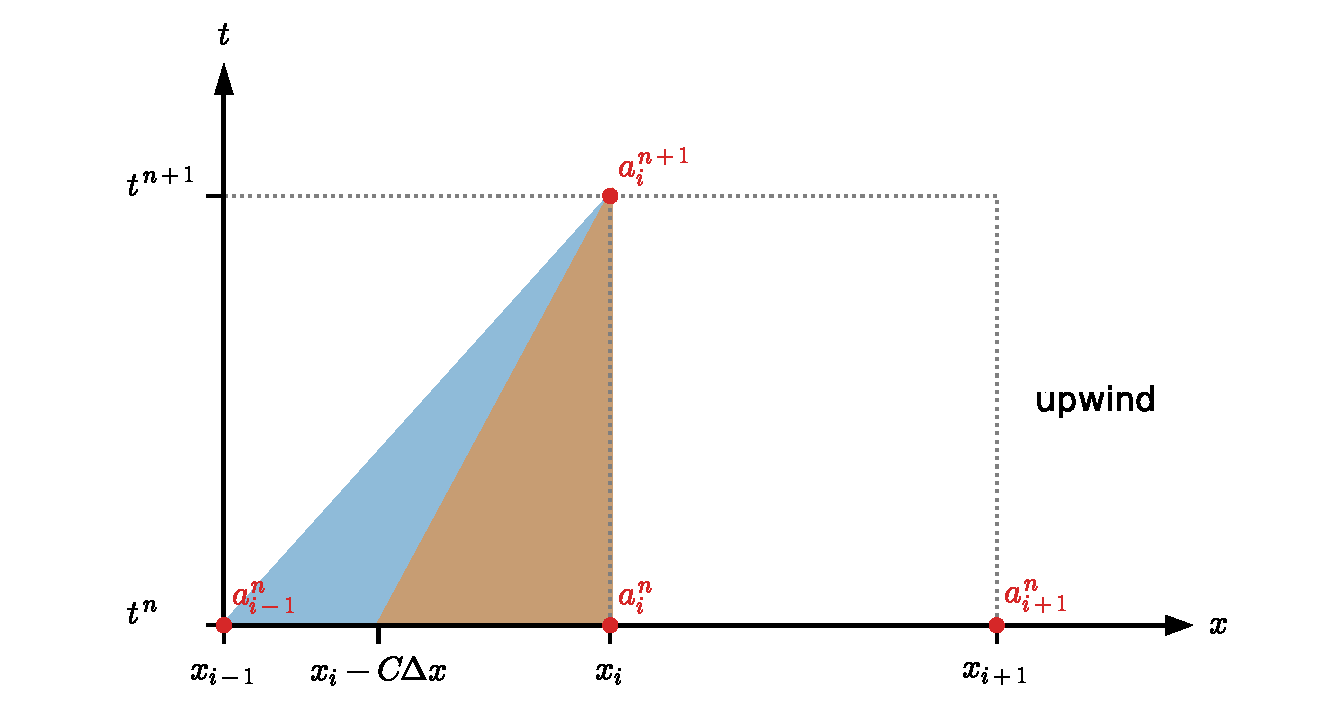
\includegraphics[width=0.7\linewidth]{domains_upwind}\\
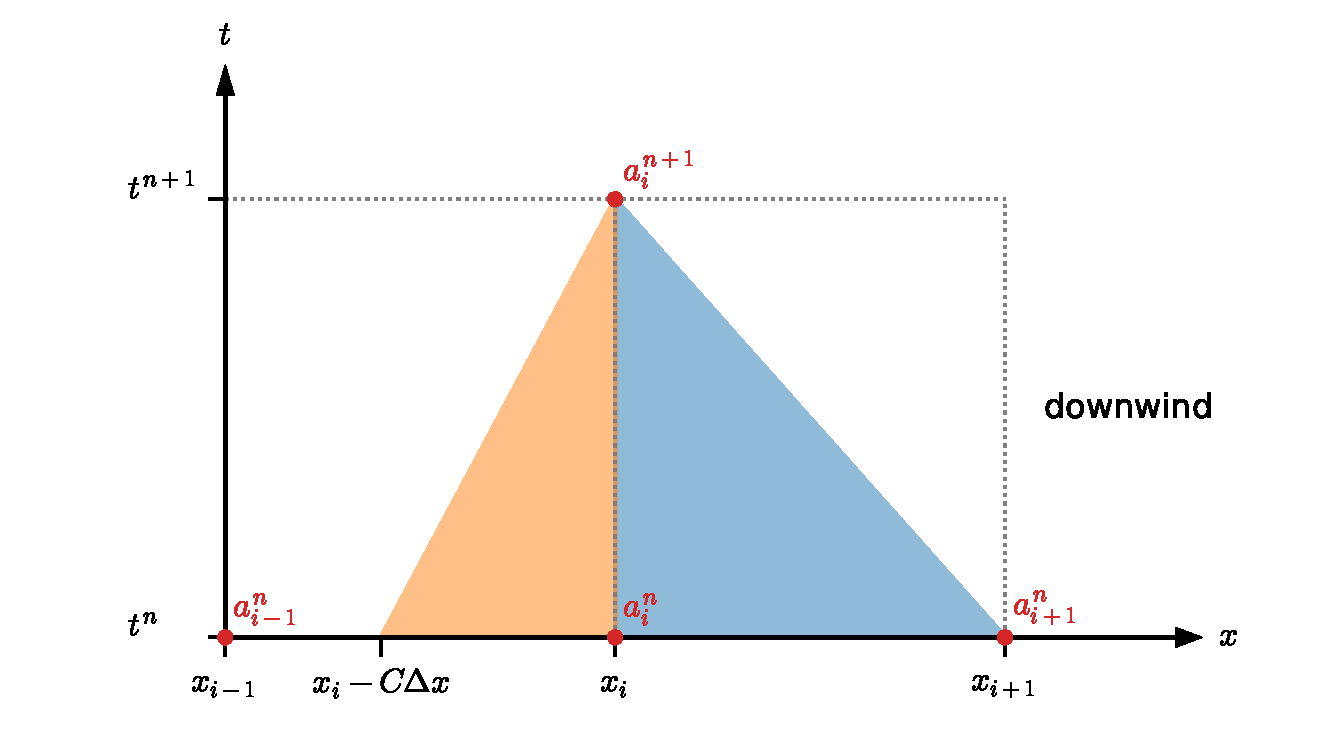
\includegraphics[width=0.7\linewidth]{domains_downwind}\\
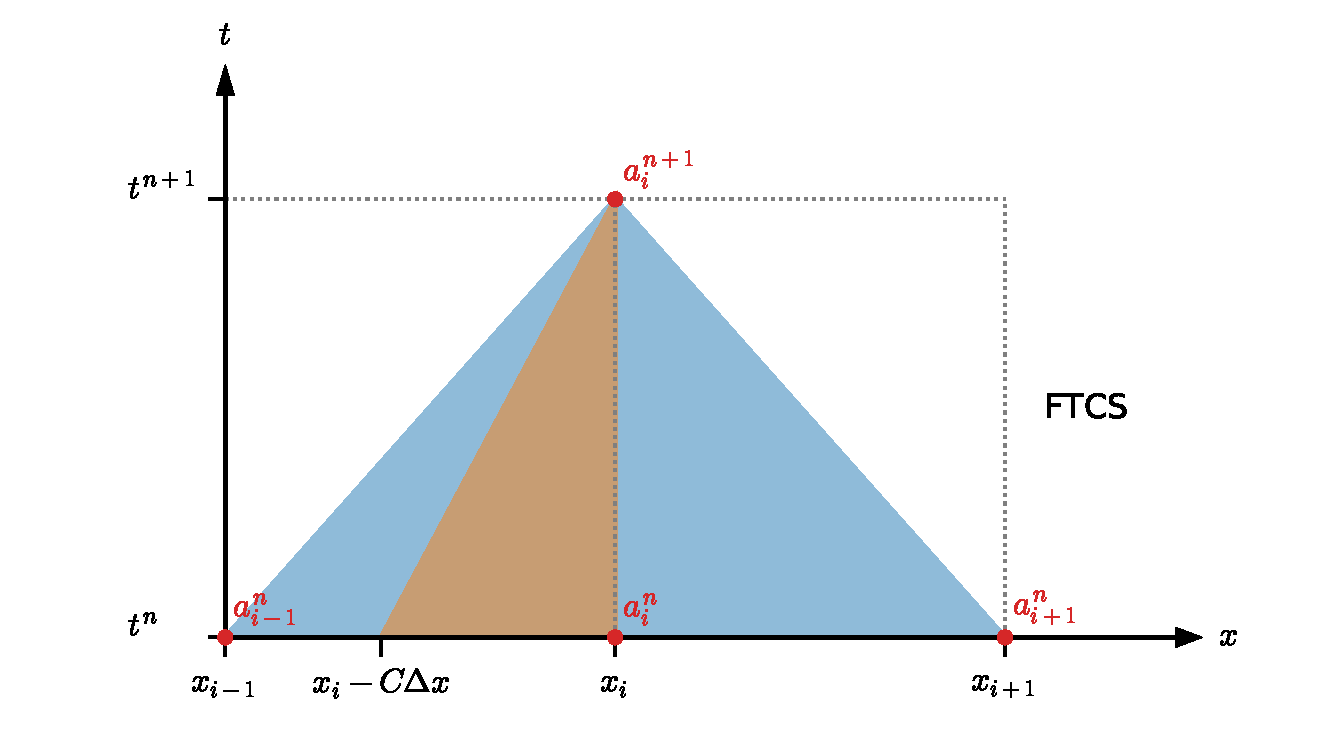
\includegraphics[width=0.7\linewidth]{domains_FTCS}
\caption[Domain of dependence space-time diagram]{\label{fig:adv:domains} Space-time diagrams showing the
  numerical domain of dependence (blue region) for three different
  difference methods.  Also show is the physical domain of
  dependence---that formed by tracing backwards from $a_i^{n+1}$ along
  a characteristic.}
\end{figure}

\section{Implicit-in-time}

An alternate approach to time-discretization is to do an implicit
discretization.  Here our upwind method would appear as:
\begin{equation}
\frac{a^{n+1}_i - a^n_i}{\Delta t} = -u \frac{a^{n+1}_i - a^{n+1}_{i-1}}{\Delta x}
\end{equation}
The only change here is that the righthand side is evaluated at the new timelevel,
$n+1$. We can write this as a linear system with coupled equations:
\begin{equation}
-\cfl a^{n+1}_{i-1} + (1 + \cfl) a^{n+1}_i = a_i^n
\end{equation}

If we use periodic boundary conditions, then point $0$ and $N-1$ are
identical, so we only need to update one of these.  Taking $a_0^{n+1} = a_{N-1}^{n+1}$, our system in matrix form appears as:
\begin{equation}
\renewcommand{\arraystretch}{1.5}
\left ( \begin{array}{ccccccc} 
1+\cfl & & & & & & -\cfl \\
-\cfl  & 1+\cfl &  \\
 &  -\cfl & 1+\cfl &  \\
 & & -\cfl & 1+\cfl &  \\
&&&\ddots&\ddots &\\
&&&&-\cfl & 1+\cfl & \\
&&&&& -\cfl &1+\cfl
\end{array}
\right )
%
\left ( \begin{array}{c}
a_1^{n+1} \\
a_2^{n+1} \\
a_3^{n+1} \\
a_4^{n+1} \\
\vdots \\
a_{N-2}^{n+1} \\
a_{N-1}^{n+1}
\end{array}
\right )
=
\left ( \begin{array}{c}
a_1^{n} \\
a_2^{n} \\
a_3^{n} \\
a_4^{n} \\
\vdots \\
a_{N-2}^{n} \\
a_{N-1}^{n}
\end{array}
\right )
\end{equation}
This requires a matrix solve---this makes implicit methods generally more
expensive than explicit methods.  However, stability analysis would show
that this implicit discretization is stable for any choice of $\cfl$. (But
one must not confuse stability with accuracy---the most accurate solutions
with this method will still have a small $\cfl$).  Also note that the form of 
the matrix will change depending on the choice of boundary conditions.
Figure~\ref{fig:fdadvect-implicit} shows the result of solving this
implicit system.

\begin{figure}[t]
\centering
% figure generated by hydro_examples/advection/fdadvect_implicit.py
\includegraphics[width=0.8\linewidth]{fdadvect-implicit}
\caption[First-order implicit finite-difference solution to linear advection]
{\label{fig:fdadvect-implicit} Finite-difference solution to the implicit first-order
finite-difference upwind method for advection, using 65 points and
a variety of CFL numbers. \\
\hydroexdoit{\href{https://github.com/zingale/hydro_examples/blob/master/advection/fdadvect_implicit.py}{fdadvect\_implicit.py}}}
\end{figure}

\begin{exercise}[Implicit advection]
{Code up the implicit advection scheme, but using outflow instead of
periodic boundary conditions.  This will change the form of the
matrix.  You can use the code from Figure~\ref{fig:fdadvect-implicit}
as a starting point.}
\end{exercise}


%%%%%%%%%%%%%%%%%%%%%%%%%%%%%%%%%%%%%%%%%%%%%%%%%%%%%%%%%%%%%%%%%%%%%%%%%%%%%%
\section{Eulerian vs.\ Lagrangian frames}

It is useful to think about how our advected quantity, $a(x,t)$, changes in
time.  The full time derivative is:
\begin{equation}
\frac{d a(x,t)}{dt} = \frac{\partial a}{\partial t} + \frac{\partial a}{\partial x}
   \frac{dx}{dt}
\end{equation}
So the value of this derivative depends on the path, $x(t)$, that we choose
to follow.  

Consider an observer who is stationary.  They will watch the flow move
past them, so $dx/dt = 0$, and $da/dt = \partial a/\partial t$.  
This fixed frame is called {\em Eulerian frame}.

Instead imagine an observer who moves with the flow, at the velocity $u$.
This way they keep pace with an individual feature in the flow and track
the changes it experiences.  In this case, $dx/dt = u$, and our derivative,
commonly written as $D/Dt$ is:
\begin{equation}
\frac{D}{Dt} = \frac{\partial}{\partial t} + u \frac{\partial}{\partial x}
\end{equation}
This is the {\em Lagrangian frame}, and the derivative, $D/Dt$ is
called the {\em Lagrangian derivative}, {\em material derivative},
{\em convective derivative}, or {\em advective
derivative}\footnote{and there are actually many more names...}.

Our linear advection equation can be written simply as $Da/Dt = 0$.
We've been solving the equations in the Eulerian frame---our grid is
fixed and the fluid moves through it.  For hydrodynamics, it will be
useful conceptually to consider the Lagrangian frame to understand how
the fluid properties change in a particular fluid element over time.


%%%%%%%%%%%%%%%%%%%%%%%%%%%%%%%%%%%%%%%%%%%%%%%%%%%%%%%%%%%%%%%%%%%%%%%%%%%%%%
\section{Errors and convergence rate}

For the advection problem (with $u>0$), the analytic solution is to
simply propagate the initial profile to the right.  This means that
with periodic boundary conditions, after advecting for one period, our
numerical solution should be identical to the initial conditions.  Any
differences are our numerical error.  We can quantify the error by
taking the norm of error\footnote{see \S~\ref{intro:sec:norm} for the
  definition of the norms} as:
\begin{equation}
\epsilon^\mathrm{abs} = \| a^\mathrm{final} - a^\mathrm{init} \|_2 \equiv
   \left [ \frac{1}{N} \sum_{i=1}^N 
   ( a_i^\mathrm{final} - a_i^\mathrm{init} )^2
  \right ]^{\myhalf}
\end{equation}
It is sometimes useful to compare to the norm of the original solution
to get a measure of the relative error:
\begin{equation}
\epsilon^\mathrm{rel} \equiv \frac{\| a^\mathrm{final} - a^\mathrm{init} \|_2}
   {\| a^\mathrm{init} \|_2}
\end{equation}
Note that for the absolute norm, it is important in these definitions
to normalize by the number of zones, $N$, otherwise our error will be
resolution-dependent.  For the relative norm, since we scale by a norm
on the same grid, this normalization will cancel.
